

\tikzset{every picture/.style={line width=0.75pt}} %set default line width to 0.75pt        

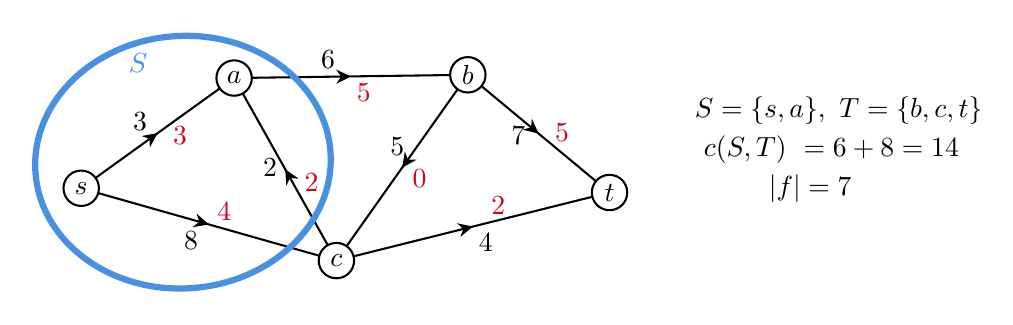
\begin{tikzpicture}[x=0.5pt,y=0.5pt,yscale=-1,xscale=1]
%uncomment if require: \path (0,210); %set diagram left start at 0, and has height of 210

%Straight Lines [id:da31781895407498073] 
\draw    (227.22,173.11) -- (322.22,38.84) ;
\draw [shift={(274.72,105.98)}, rotate = 305.28] [fill={rgb, 255:red, 0; green, 0; blue, 0 }  ][line width=0.08]  [draw opacity=0] (10.72,-5.15) -- (0,0) -- (10.72,5.15) -- (7.12,0) -- cycle    ;
%Straight Lines [id:da3853598268579197] 
\draw    (153.31,41.18) -- (227.22,173.11) ;
\draw [shift={(190.27,107.14)}, rotate = 60.74] [fill={rgb, 255:red, 0; green, 0; blue, 0 }  ][line width=0.08]  [draw opacity=0] (10.72,-5.15) -- (0,0) -- (10.72,5.15) -- (7.12,0) -- cycle    ;
%Straight Lines [id:da14604600957867897] 
\draw    (42.79,120.83) -- (227.22,173.11) ;
\draw [shift={(135.01,146.97)}, rotate = 195.83] [fill={rgb, 255:red, 0; green, 0; blue, 0 }  ][line width=0.08]  [draw opacity=0] (10.72,-5.15) -- (0,0) -- (10.72,5.15) -- (7.12,0) -- cycle    ;
%Straight Lines [id:da8640956582518242] 
\draw    (424.62,123.9) -- (227.22,173.11) ;
\draw [shift={(325.92,148.5)}, rotate = 166] [fill={rgb, 255:red, 0; green, 0; blue, 0 }  ][line width=0.08]  [draw opacity=0] (10.72,-5.15) -- (0,0) -- (10.72,5.15) -- (7.12,0) -- cycle    ;
%Straight Lines [id:da285469110869773] 
\draw    (42.79,120.83) -- (153.31,41.18) ;
\draw [shift={(98.05,81)}, rotate = 504.22] [fill={rgb, 255:red, 0; green, 0; blue, 0 }  ][line width=0.08]  [draw opacity=0] (10.72,-5.15) -- (0,0) -- (10.72,5.15) -- (7.12,0) -- cycle    ;
%Straight Lines [id:da8162300663234149] 
\draw    (322.22,38.84) -- (424.62,123.9) ;
\draw [shift={(373.42,81.37)}, rotate = 219.71] [fill={rgb, 255:red, 0; green, 0; blue, 0 }  ][line width=0.08]  [draw opacity=0] (10.72,-5.15) -- (0,0) -- (10.72,5.15) -- (7.12,0) -- cycle    ;
%Straight Lines [id:da5085854502811855] 
\draw    (153.31,41.18) -- (322.22,38.84) ;
\draw [shift={(237.76,40.01)}, rotate = 539.21] [fill={rgb, 255:red, 0; green, 0; blue, 0 }  ][line width=0.08]  [draw opacity=0] (10.72,-5.15) -- (0,0) -- (10.72,5.15) -- (7.12,0) -- cycle    ;
%Shape: Ellipse [id:dp651117123053256] 
\draw  [fill={rgb, 255:red, 255; green, 255; blue, 255 }  ,fill opacity=1 ] (30,120.83) .. controls (30,113.77) and (35.73,108.04) .. (42.79,108.04) .. controls (49.86,108.04) and (55.58,113.77) .. (55.58,120.83) .. controls (55.58,127.9) and (49.86,133.62) .. (42.79,133.62) .. controls (35.73,133.62) and (30,127.9) .. (30,120.83) -- cycle ;
%Shape: Ellipse [id:dp7399561756845123] 
\draw  [fill={rgb, 255:red, 255; green, 255; blue, 255 }  ,fill opacity=1 ] (140.52,41.18) .. controls (140.52,34.11) and (146.25,28.39) .. (153.31,28.39) .. controls (160.38,28.39) and (166.1,34.11) .. (166.1,41.18) .. controls (166.1,48.24) and (160.38,53.97) .. (153.31,53.97) .. controls (146.25,53.97) and (140.52,48.24) .. (140.52,41.18) -- cycle ;
%Shape: Ellipse [id:dp8268258265249401] 
\draw  [fill={rgb, 255:red, 255; green, 255; blue, 255 }  ,fill opacity=1 ] (309.43,38.84) .. controls (309.43,31.78) and (315.15,26.05) .. (322.22,26.05) .. controls (329.28,26.05) and (335.01,31.78) .. (335.01,38.84) .. controls (335.01,45.9) and (329.28,51.63) .. (322.22,51.63) .. controls (315.15,51.63) and (309.43,45.9) .. (309.43,38.84) -- cycle ;
%Shape: Ellipse [id:dp5421818862330341] 
\draw  [fill={rgb, 255:red, 255; green, 255; blue, 255 }  ,fill opacity=1 ] (214.43,173.11) .. controls (214.43,166.05) and (220.15,160.32) .. (227.22,160.32) .. controls (234.28,160.32) and (240.01,166.05) .. (240.01,173.11) .. controls (240.01,180.18) and (234.28,185.9) .. (227.22,185.9) .. controls (220.15,185.9) and (214.43,180.18) .. (214.43,173.11) -- cycle ;
%Shape: Ellipse [id:dp031187496945339066] 
\draw  [fill={rgb, 255:red, 255; green, 255; blue, 255 }  ,fill opacity=1 ] (411.83,123.9) .. controls (411.83,116.83) and (417.56,111.11) .. (424.62,111.11) .. controls (431.69,111.11) and (437.41,116.83) .. (437.41,123.9) .. controls (437.41,130.96) and (431.69,136.69) .. (424.62,136.69) .. controls (417.56,136.69) and (411.83,130.96) .. (411.83,123.9) -- cycle ;
%Shape: Ellipse [id:dp3896768851761181] 
\draw  [color={rgb, 255:red, 74; green, 144; blue, 226 }  ,draw opacity=1 ][line width=2.25]  (110.27,10.95) .. controls (169.16,7.03) and (219.61,44.6) .. (222.96,94.88) .. controls (226.31,145.15) and (181.28,189.09) .. (122.39,193.01) .. controls (63.51,196.93) and (13.05,159.35) .. (9.71,109.08) .. controls (6.36,58.8) and (51.38,14.87) .. (110.27,10.95) -- cycle ;

% Text Node
\draw (42.79,120.83) node   [align=left] {$\displaystyle s$};
% Text Node
\draw (153.31,41.18) node   [align=left] {$\displaystyle a$};
% Text Node
\draw (322.22,38.84) node   [align=left] {$\displaystyle b$};
% Text Node
\draw (227.22,173.11) node   [align=left] {$\displaystyle c$};
% Text Node
\draw (424.62,123.9) node   [align=left] {$\displaystyle t$};
% Text Node
\draw (115,150) node [anchor=north west][inner sep=0.75pt]   [align=left] {$\displaystyle 8$};
% Text Node
\draw (264,82) node [anchor=north west][inner sep=0.75pt]   [align=left] {$\displaystyle 5$};
% Text Node
\draw (172,97) node [anchor=north west][inner sep=0.75pt]   [align=left] {$\displaystyle 2$};
% Text Node
\draw (78,64) node [anchor=north west][inner sep=0.75pt]   [align=left] {$\displaystyle 3$};
% Text Node
\draw (327.92,151.5) node [anchor=north west][inner sep=0.75pt]   [align=left] {$\displaystyle 4$};
% Text Node
\draw (351.42,74.37) node [anchor=north west][inner sep=0.75pt]   [align=left] {$\displaystyle 7$};
% Text Node
\draw (214,19) node [anchor=north west][inner sep=0.75pt]   [align=left] {$\displaystyle 6$};
% Text Node
\draw (490.5,80.5) node [anchor=north west][inner sep=0.75pt]   [align=left] {$\displaystyle c( S,T) \ =6+8=14$};
% Text Node
\draw (484,52.5) node [anchor=north west][inner sep=0.75pt]   [align=left] {$\displaystyle S=\{s,a\} ,\ T=\{b,c,t\}$};
% Text Node
\draw (139,129) node [anchor=north west][inner sep=0.75pt]   [align=left] {$\displaystyle \textcolor[rgb]{0.82,0.01,0.11}{4}$};
% Text Node
\draw (202,108) node [anchor=north west][inner sep=0.75pt]   [align=left] {$\displaystyle \textcolor[rgb]{0.82,0.01,0.11}{2}$};
% Text Node
\draw (337,125) node [anchor=north west][inner sep=0.75pt]   [align=left] {$\displaystyle \textcolor[rgb]{0.82,0.01,0.11}{2}$};
% Text Node
\draw (107,74) node [anchor=north west][inner sep=0.75pt]   [align=left] {$\displaystyle \textcolor[rgb]{0.82,0.01,0.11}{3}$};
% Text Node
\draw (239.76,43.01) node [anchor=north west][inner sep=0.75pt]   [align=left] {$\displaystyle \textcolor[rgb]{0.82,0.01,0.11}{5}$};
% Text Node
\draw (280,105) node [anchor=north west][inner sep=0.75pt]   [align=left] {$\displaystyle \textcolor[rgb]{0.82,0.01,0.11}{0}$};
% Text Node
\draw (383,72) node [anchor=north west][inner sep=0.75pt]   [align=left] {$\displaystyle \textcolor[rgb]{0.82,0.01,0.11}{5}$};
% Text Node
\draw (537.5,108.5) node [anchor=north west][inner sep=0.75pt]   [align=left] {$\displaystyle | f|=7$};
% Text Node
\draw (75,21) node [anchor=north west][inner sep=0.75pt]   [align=left] {$\displaystyle \textcolor[rgb]{0.29,0.56,0.89}{S}$};


\end{tikzpicture}

